\chapter{Interview results}
\label{ch:interviewresults}

\section{Interviews}
\label{sec:interviews}
The interviews are in the format of semi-structured. I used a minimal set of questions. Based on the answers, the technique of hitchhiking was applied when there was a suspicion of extra information about \acrshort{ea} and \gls{antifragile} attributes. The interview summaries can be found in \cref{app:interviewsummaries}.

\begin{table}[!h]
	\label{tab:interviewquestions}
	\begin{center}
			\begin{tabular}{@{}p{0.1\textwidth}p{0.75\textwidth}p{0.15\textwidth}@{}}
				\toprule
				\textbf{Number} & \textbf{Question} & \textbf{Concept} \\ \midrule %
				1a. & How is your organisation applying \acrshort{ea}? & \acrshort{ea} \\%
				1b. & Who is accountable for \acrshort{ea} in your organisation? & \acrshort{ea} \\%
				1c. & How is \acrshort{ea} enabling your organisation to quickly adapt to changes (external influences)? & \acrshort{ea} \\%
				2a. & Does the operational model of the\gls{ps} \gls{foster} \gls{agility}? & \Gls{antifragile} \\%
				2b. & How is the \acrshort{ea} of your organisation contributing to \gls{foster} \gls{agility} in the \gls{ps}? & \acrshort{ea} \\%
				3a. & How does the public sector deal with \gls{uncertainty}? & \Gls{antifragile} \\%
				3b. & How is the \acrshort{ea} of your organisation contributing to dealing with \gls{uncertainty} in the \gls{ps}?
				 & \acrshort{ea} \\%
				4a. & How is the public sector dealing with unexpected events? & \Gls{antifragile} \\%
				4b. & How is \acrshort{ea} of your organisation contributing to dealing with unexpected events in the \gls{ps}? & \acrshort{ea} \\%
				5a. & Could you describe the risk appetite of the \gls{ps}? & \Gls{antifragile} \\%
				5b. & How does the \acrshort{ea} of your organisation match the risk appetite of the \gls{ps}?
				  & \acrshort{ea} \\%
				6a. & How is \gls{diversity} and \gls{optionality} used in the \gls{ps}? & \Gls{antifragile} \\%
				6b. & How does \acrshort{ea} of your organisation support \gls{diversity} and \gls{optionality} in the \gls{ps}? & \acrshort{ea} \\%																								
				Closing & Did you miss an important subject or do you want to add something else? & non-specific \\%
				\bottomrule
			\end{tabular}
		\caption{Interview questions}
	\end{center}
\end{table}

\section{Summary of interviews}

\section{interview results}
\subsection{Engineering Resilience}
\begin{figure}[H]
	\centering
	\begin{subfigure}[H]{0.5\textwidth}
		\centering
		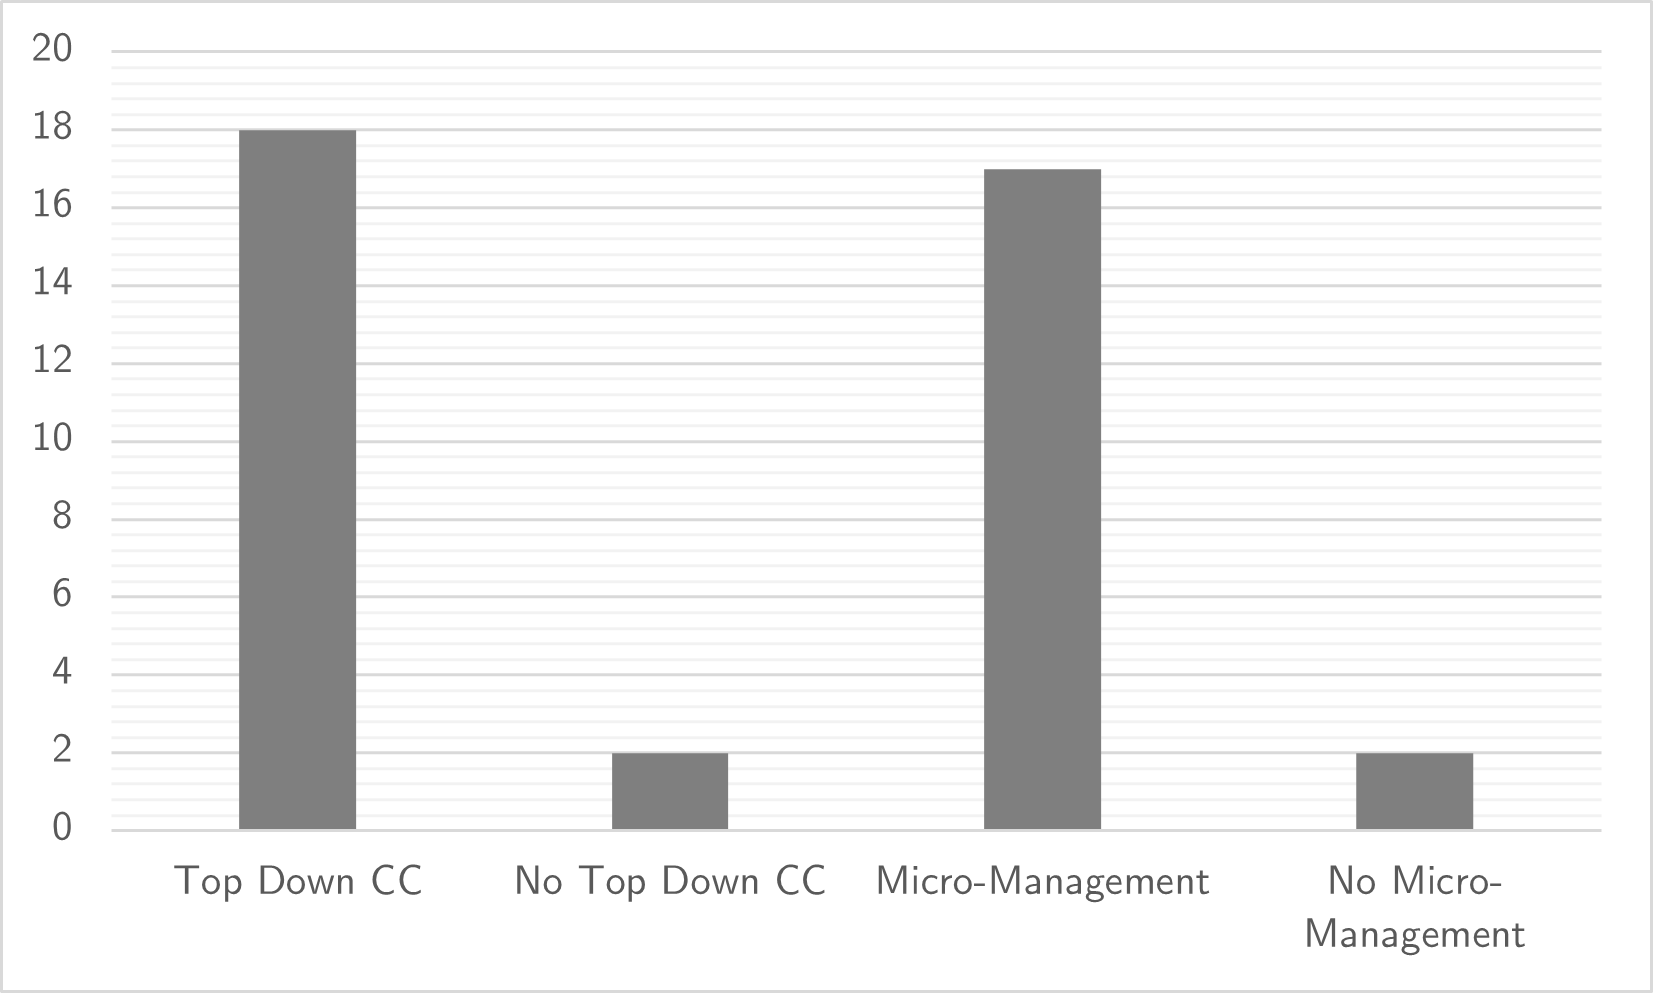
\includegraphics[width=0.95\linewidth]{images/engineeringresilience_frequency}
		\caption{Engineering Resilience Frequency}
		\label{fig:engineeringresiliencefrequency}
	\end{subfigure}%
	\begin{subfigure}[H]{0.5\textwidth}
		\centering
		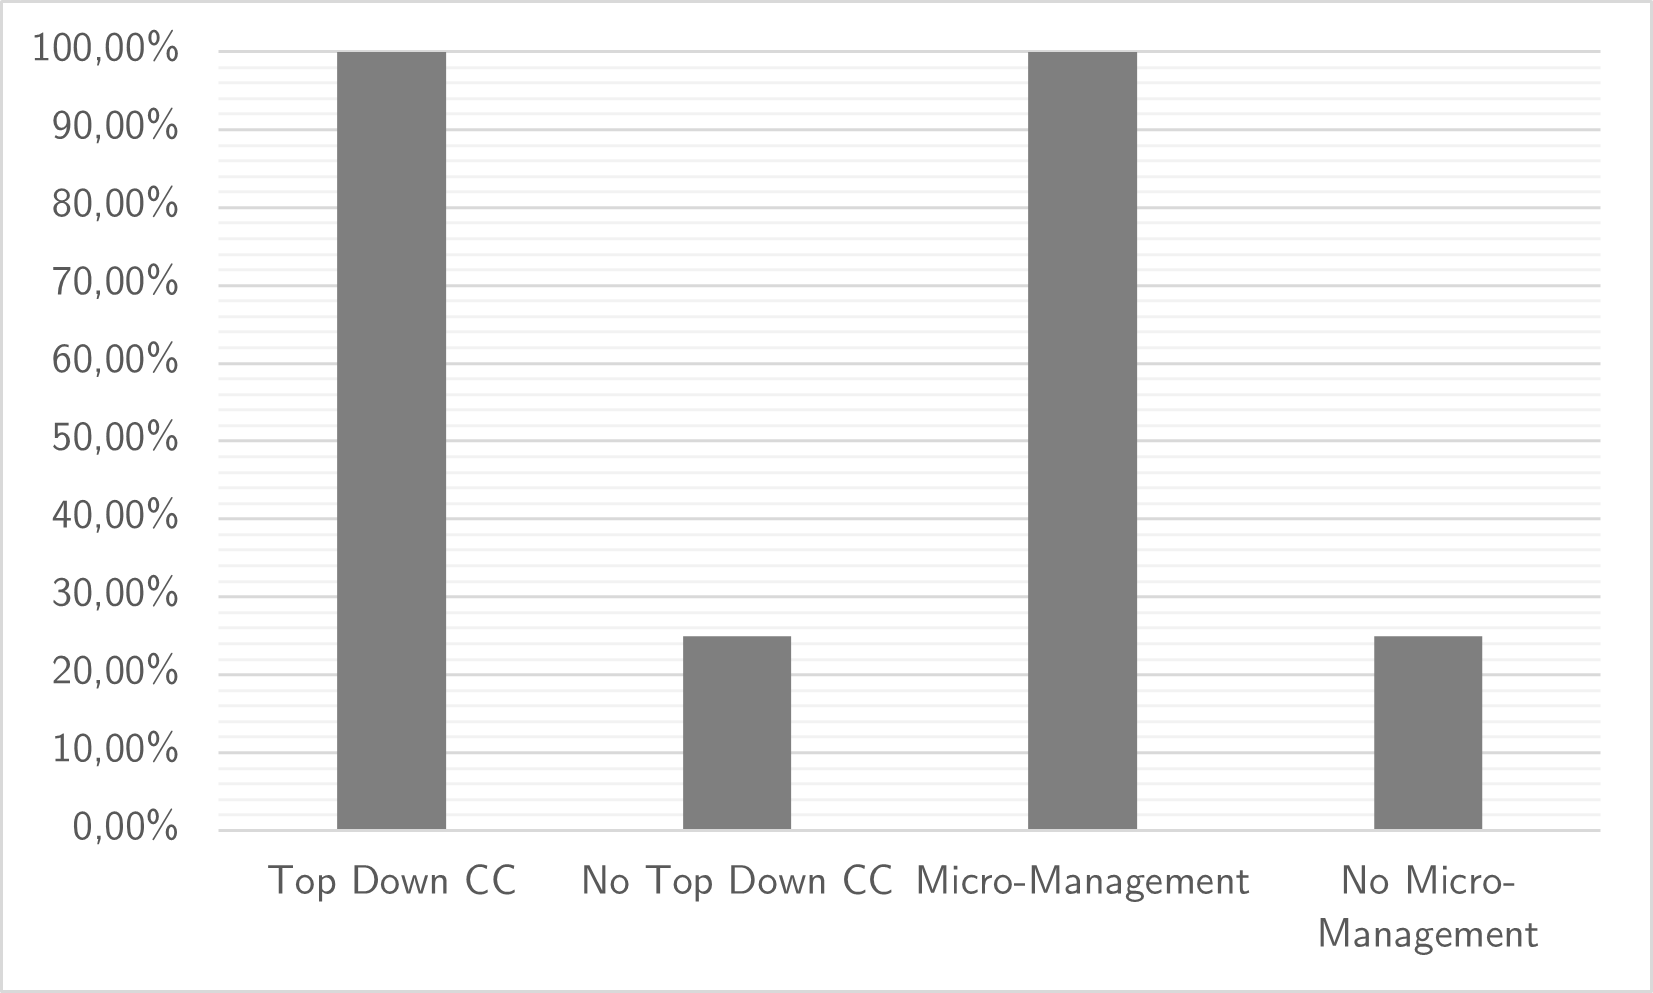
\includegraphics[width=0.95\linewidth]{images/engineeringresilience_cases}
		\caption{Engineering Resilience \% Cases}
		\label{fig:engineeringresiliencecases}
	\end{subfigure}
	\caption{Interview results Engineering Resilience}
	\label{fig:interviewresultsengineeringresilience}
\end{figure}

\subsection{Systems Resilience}
\begin{figure}[H]
	\centering
	\begin{subfigure}[H]{0.5\textwidth}
		\centering
		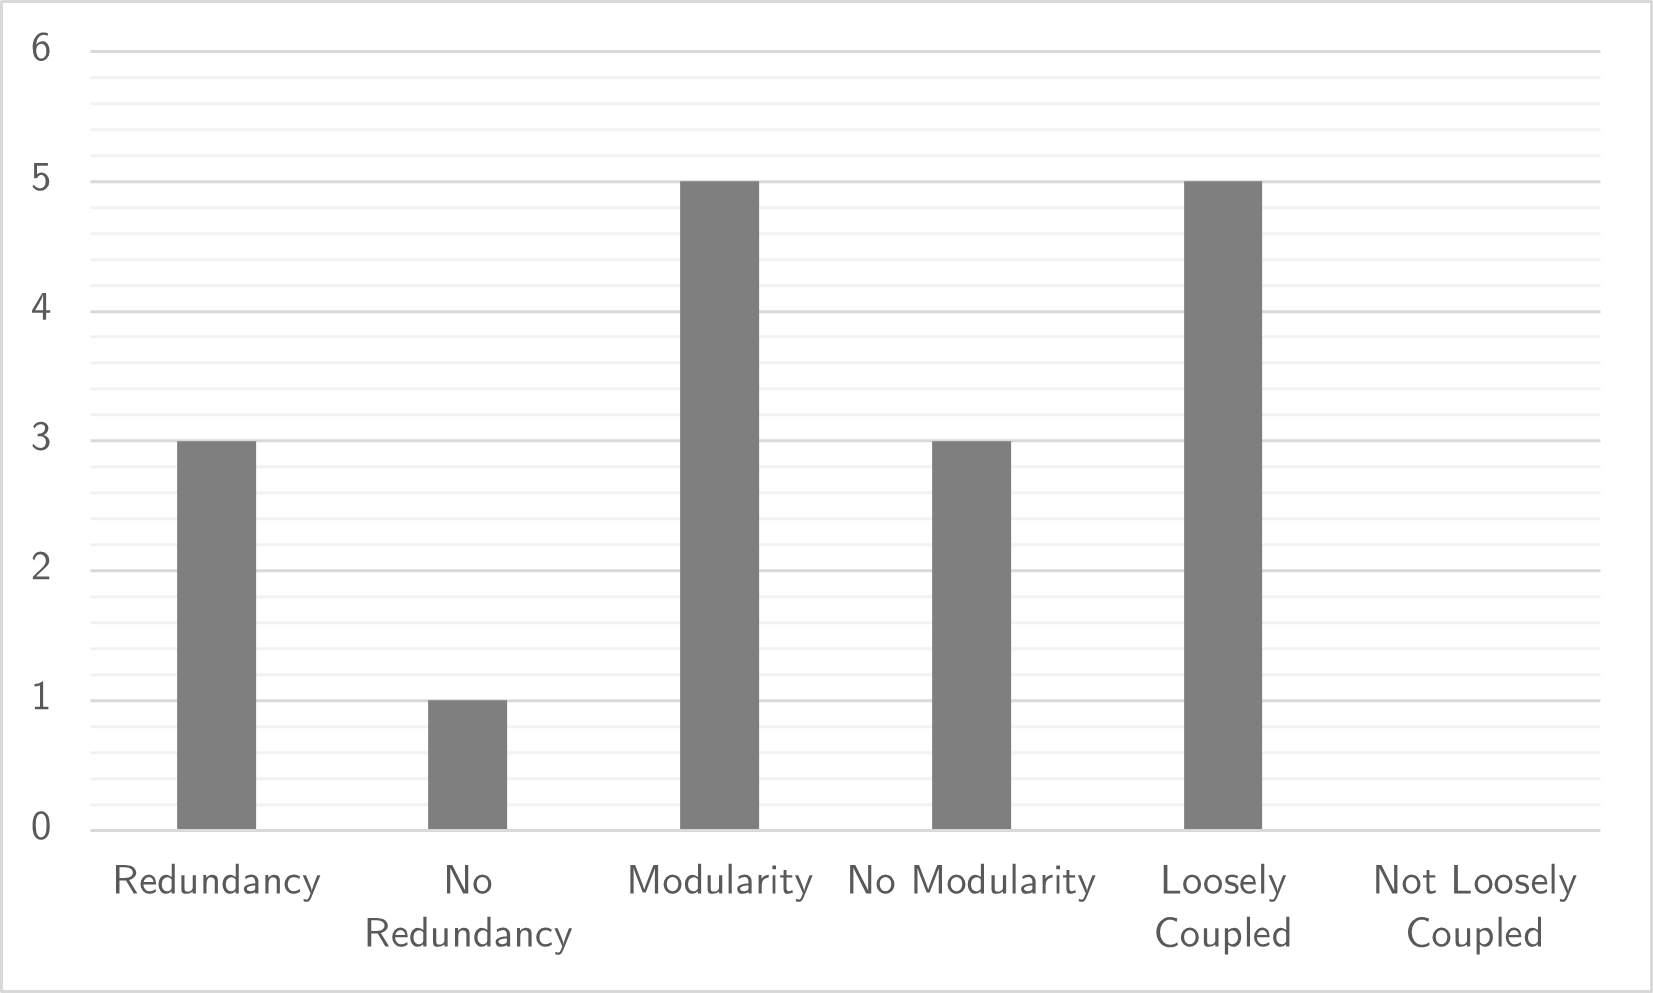
\includegraphics[width=0.95\linewidth]{images/systemsresilience_frequency}
		\caption{Systems Resilience Frequency}
		\label{fig:systemsresiliencefrequency}
	\end{subfigure}%
	\begin{subfigure}[H]{0.5\textwidth}
		\centering
		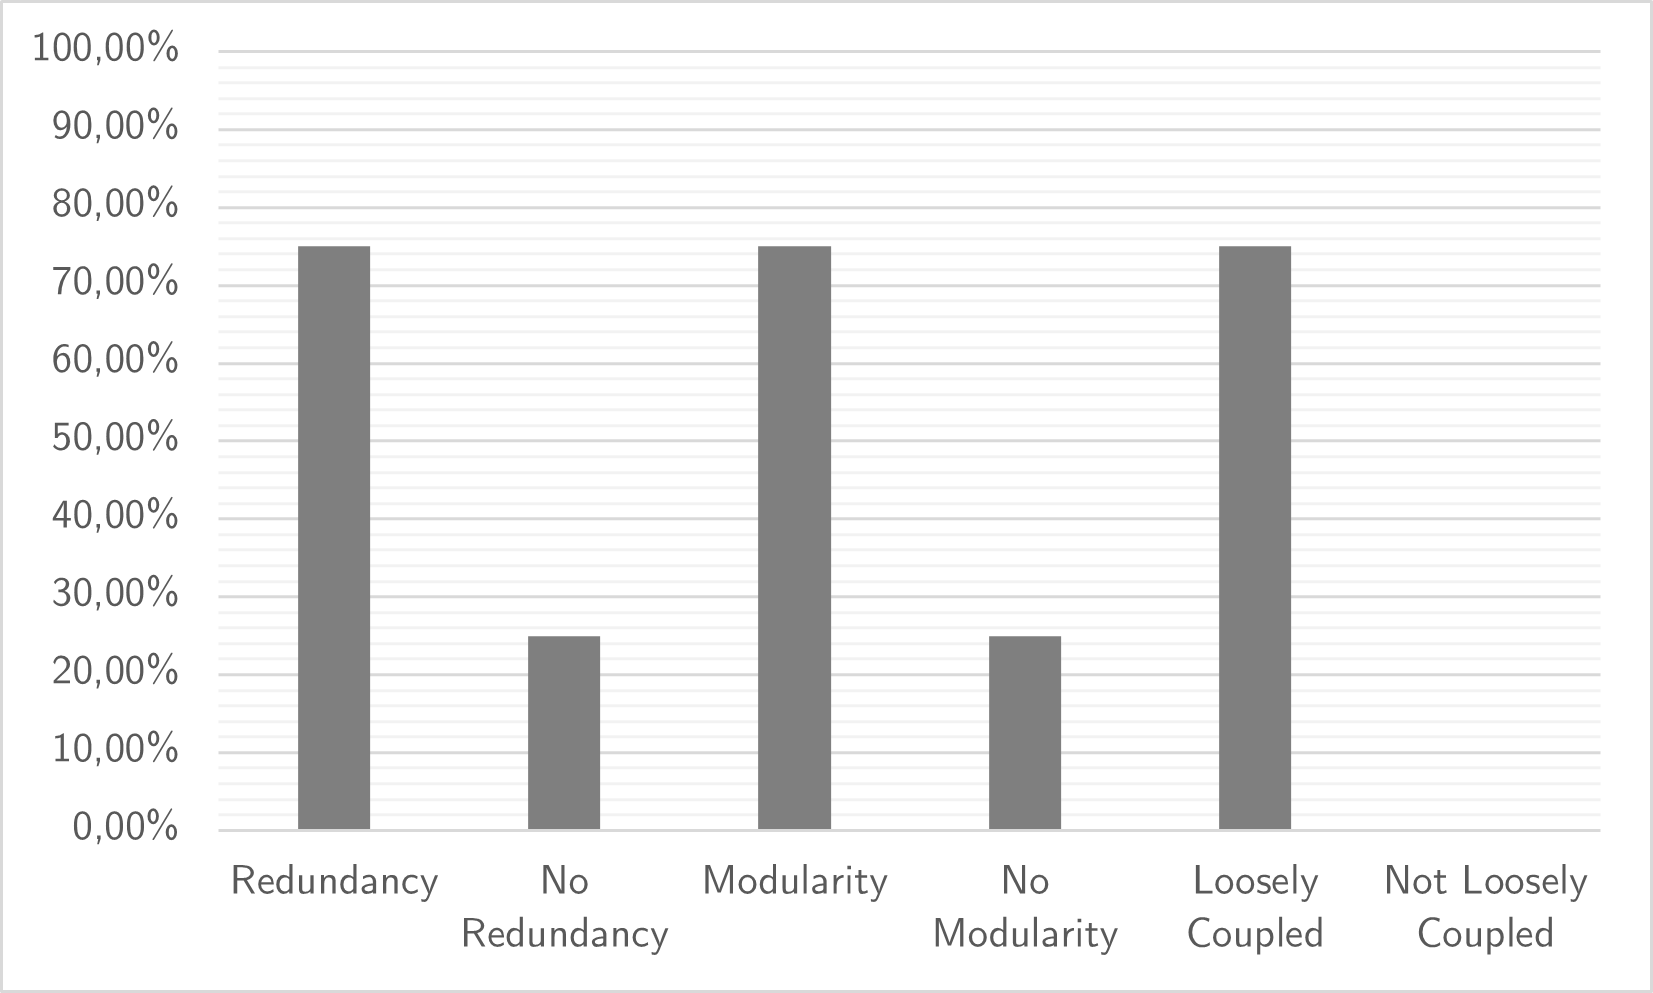
\includegraphics[width=0.95\linewidth]{images/systemsresilience_cases}
		\caption{Systems Resilience \% Cases}
		\label{fig:systemsresiliencecases}
	\end{subfigure}
	\caption{Interview results Systems Resilience}
	\label{fig:interviewresultssystemsresilience}
\end{figure}

\subsection{Complex Adaptive System Resilience}
\begin{figure}[H]
	\centering
	\begin{subfigure}[H]{0.5\textwidth}
		\centering
		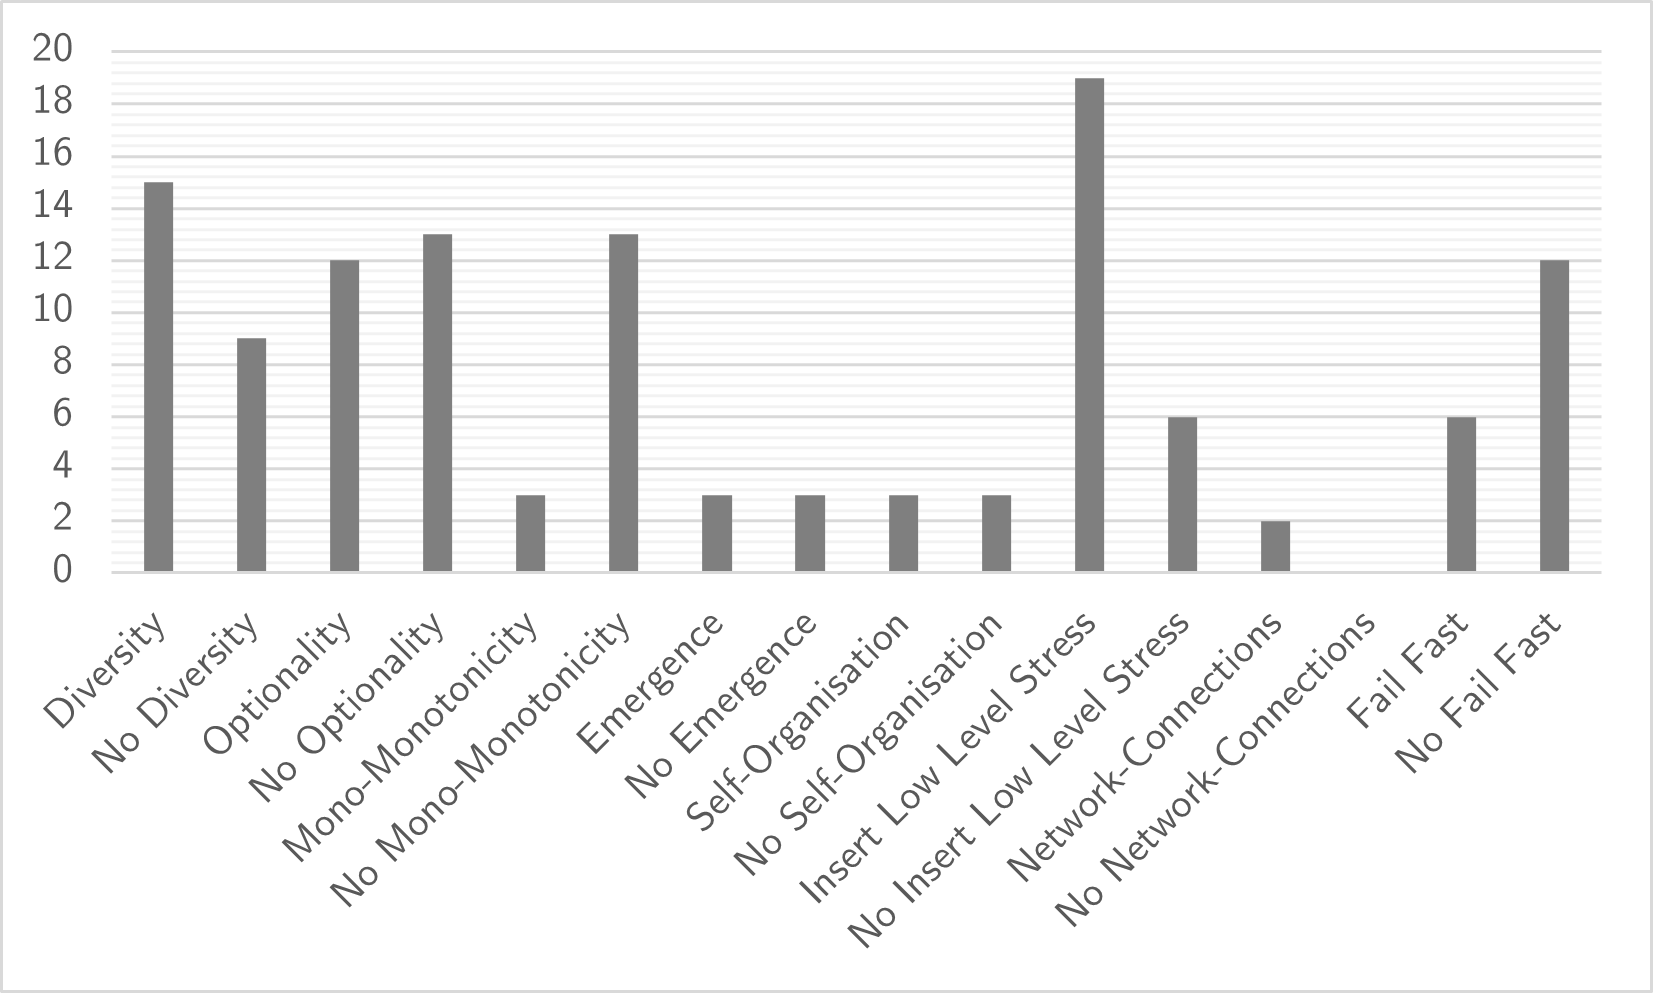
\includegraphics[width=0.95\linewidth]{images/cas_frequency}
		\caption{CAS Resilience Frequency}
		\label{fig:casfrequency}
	\end{subfigure}%
	\begin{subfigure}[H]{0.5\textwidth}
		\centering
		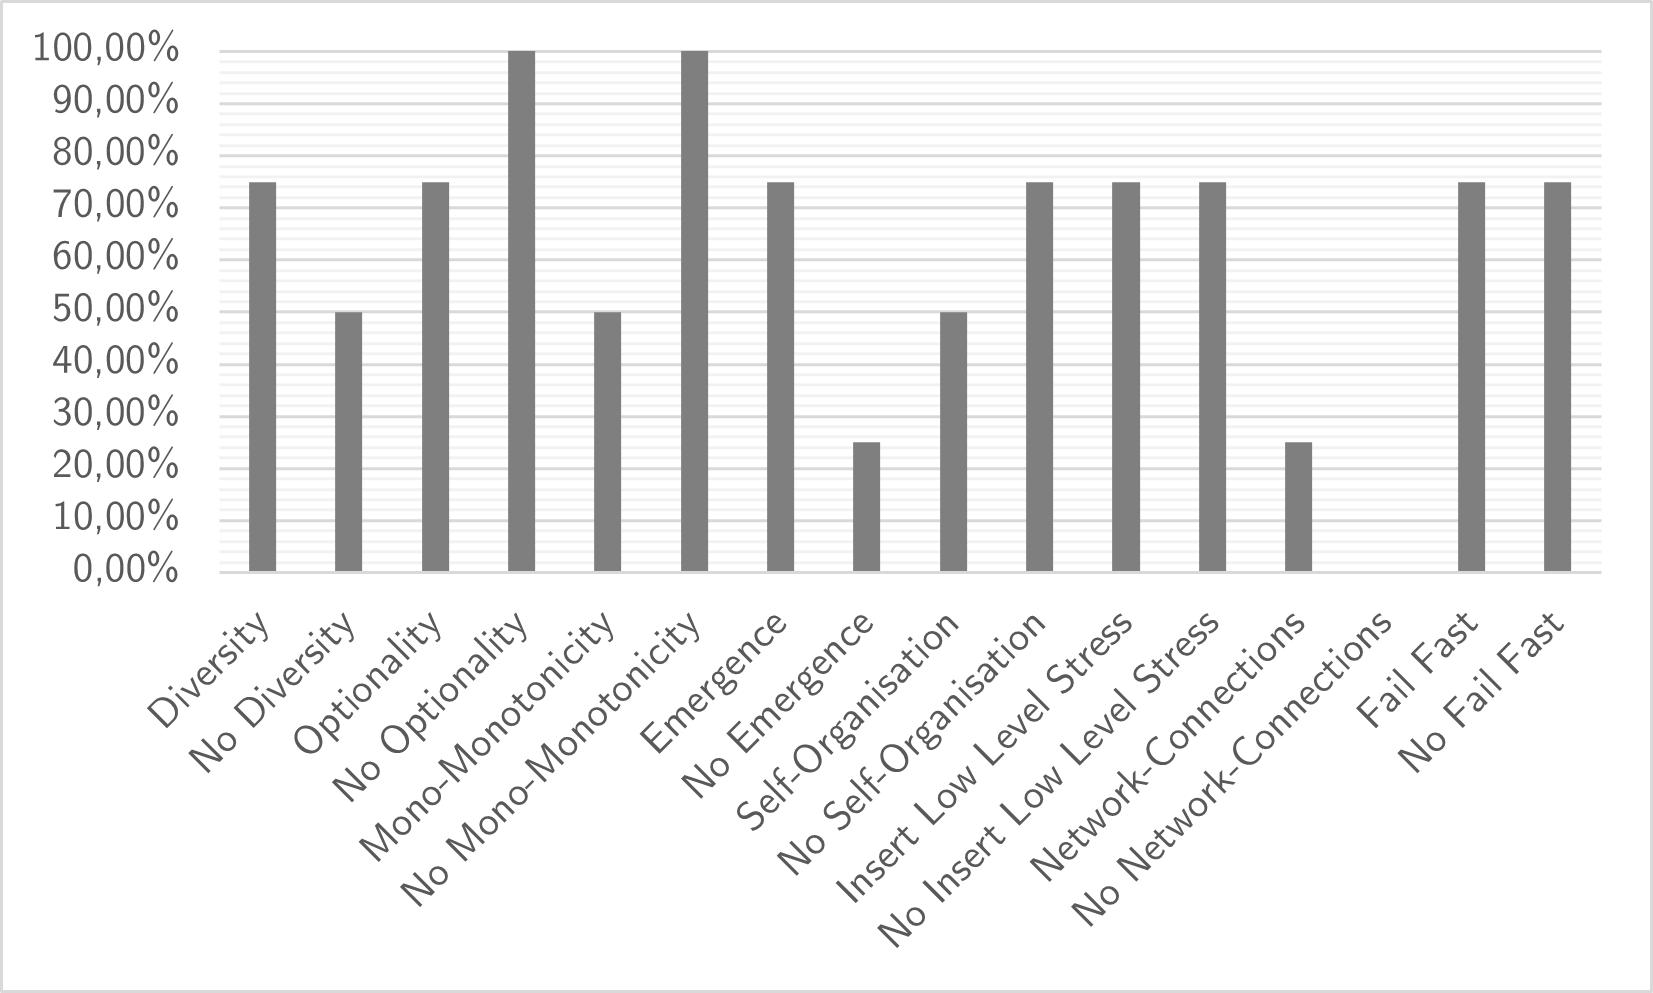
\includegraphics[width=0.95\linewidth]{images/cas_cases}
		\caption{CAS Resilience \% Cases}
		\label{fig:cascases}
	\end{subfigure}
	\caption{Interview results CAS Resilience}
	\label{fig:interviewresultscas}
\end{figure}
\subsection{Antifragile}
\begin{figure}[H]
	\centering
	\begin{subfigure}[H]{0.5\textwidth}
		\centering
		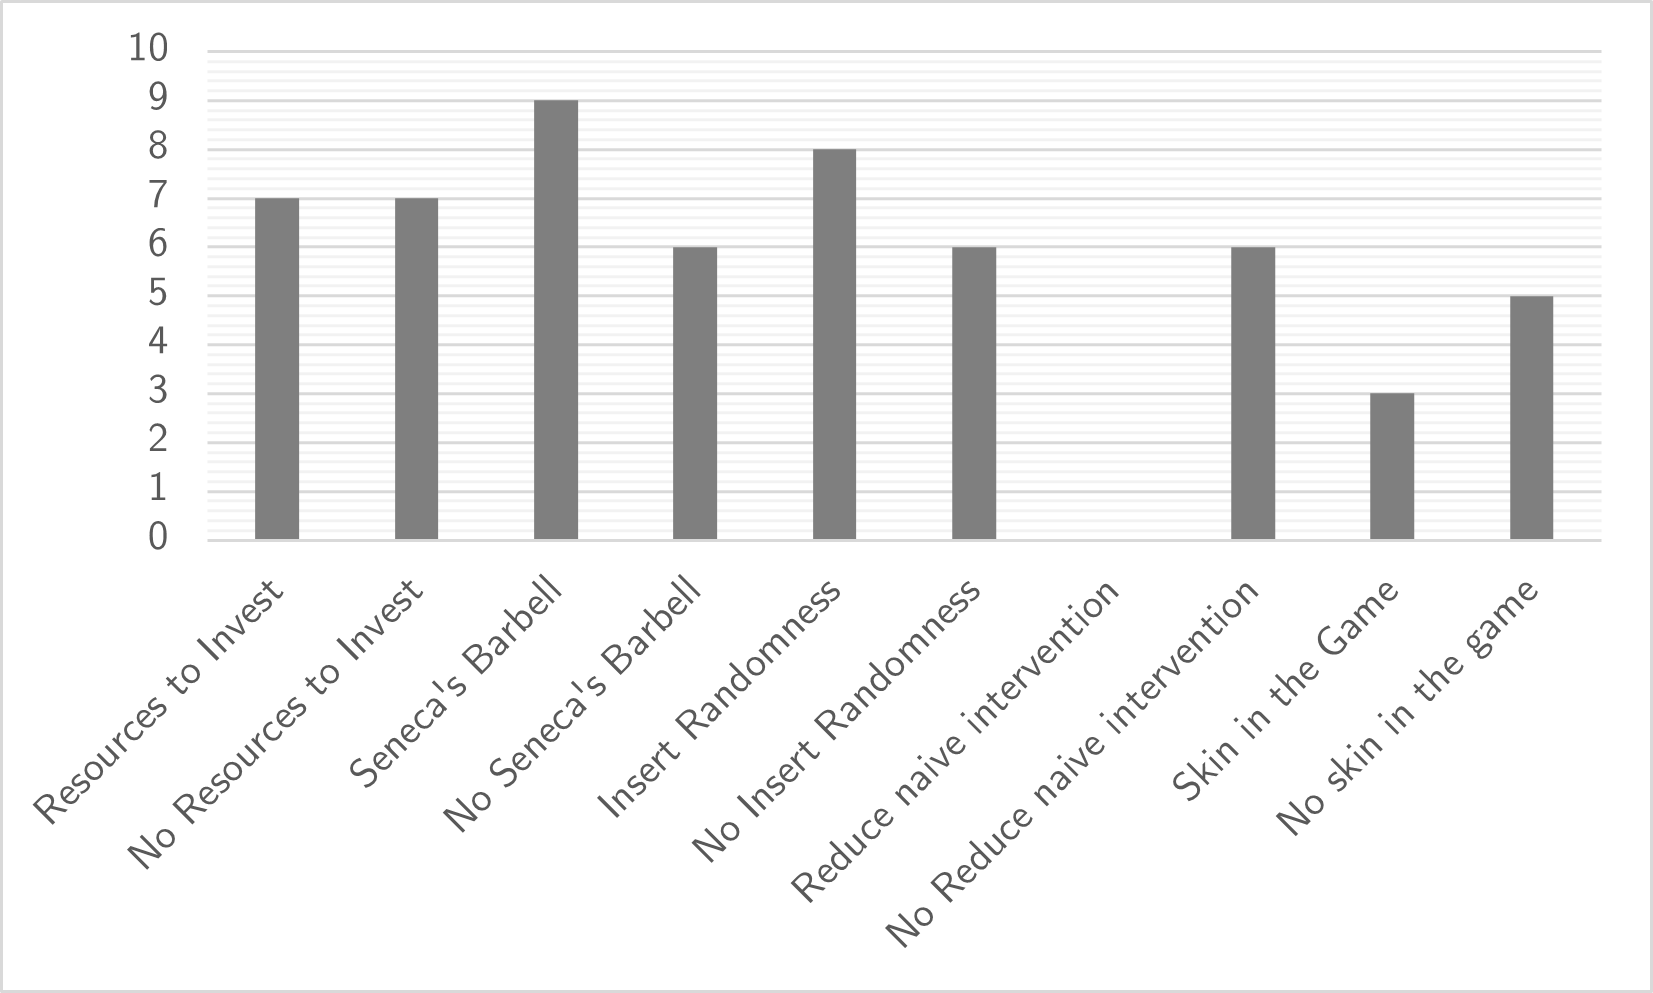
\includegraphics[width=0.95\linewidth]{images/antifragile_frequency}
		\caption{Antifragile Frequency}
		\label{fig:antifragilefrequency}
	\end{subfigure}%
	\begin{subfigure}[H]{0.5\textwidth}
		\centering
		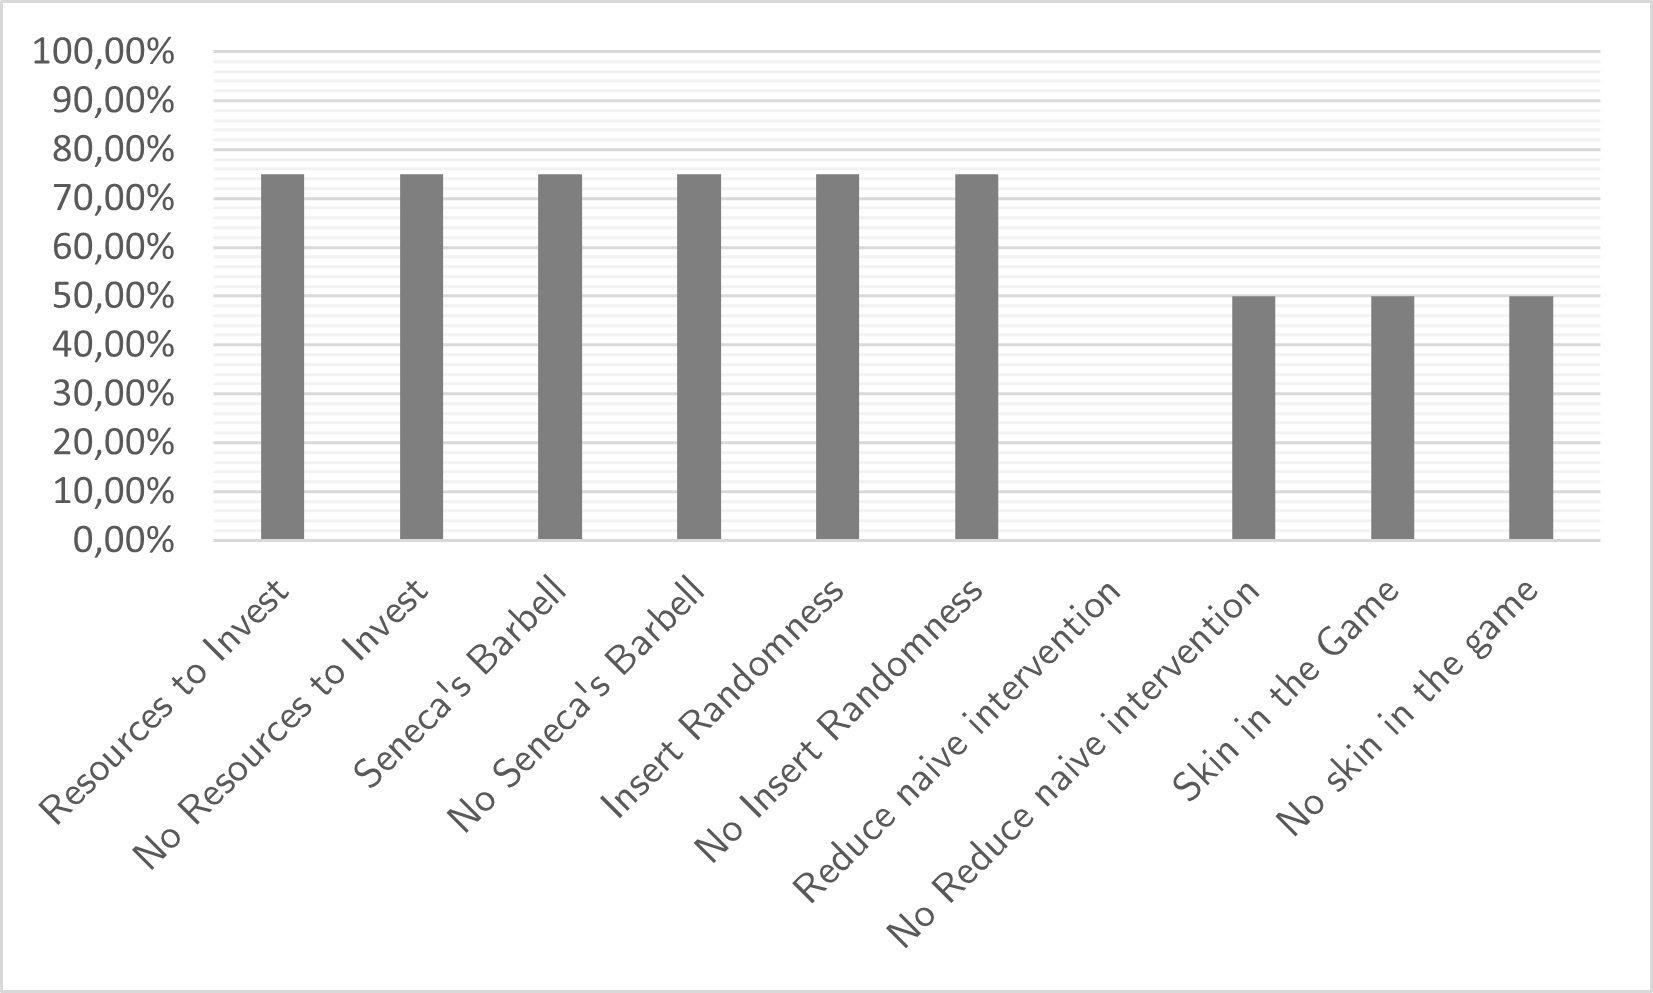
\includegraphics[width=0.95\linewidth]{images/antifragile_cases}
		\caption{Antifragile \% of Cases}
		\label{fig:antifragilecases}
	\end{subfigure}
	\caption{Interview results Antifragile}
	\label{fig:interviewresultsantifragile}
\end{figure}
\subsection{Learning organisation}
\begin{figure}[H]
	\centering
	\begin{subfigure}[H]{0.5\textwidth}
		\centering
		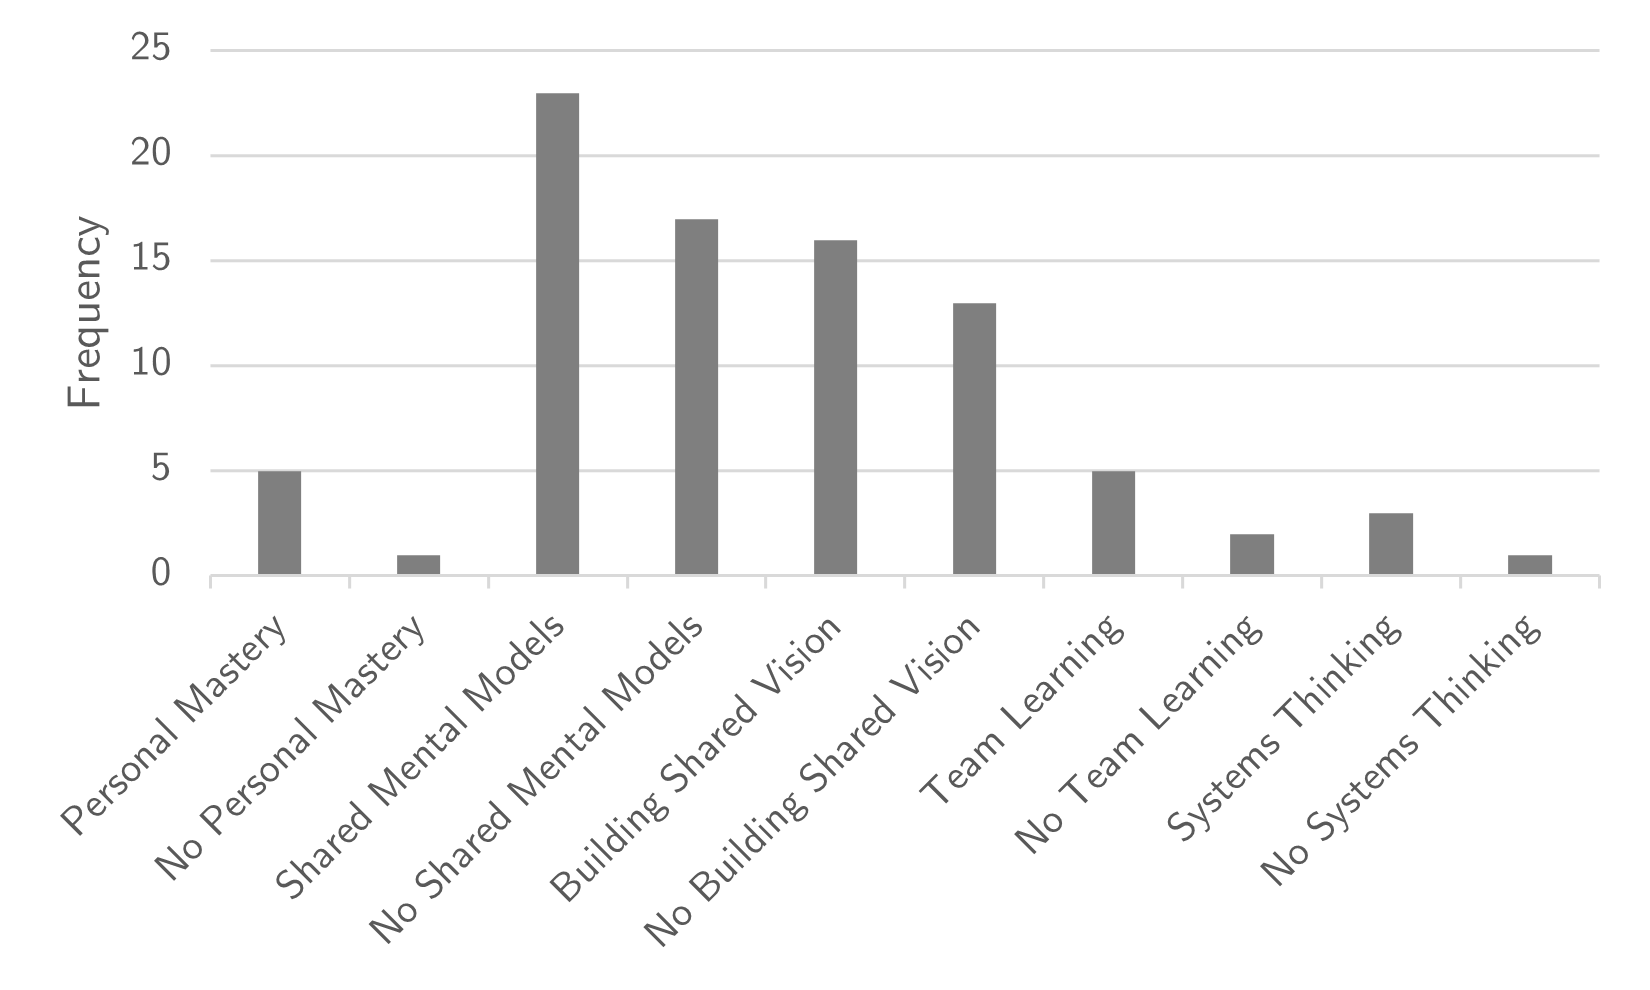
\includegraphics[width=0.95\linewidth]{images/learningorganisation_frequency}
		\caption{Learning Organisation Frequency}
		\label{fig:learningorganisationfrequency}
	\end{subfigure}%
	\begin{subfigure}[H]{0.5\textwidth}
		\centering
		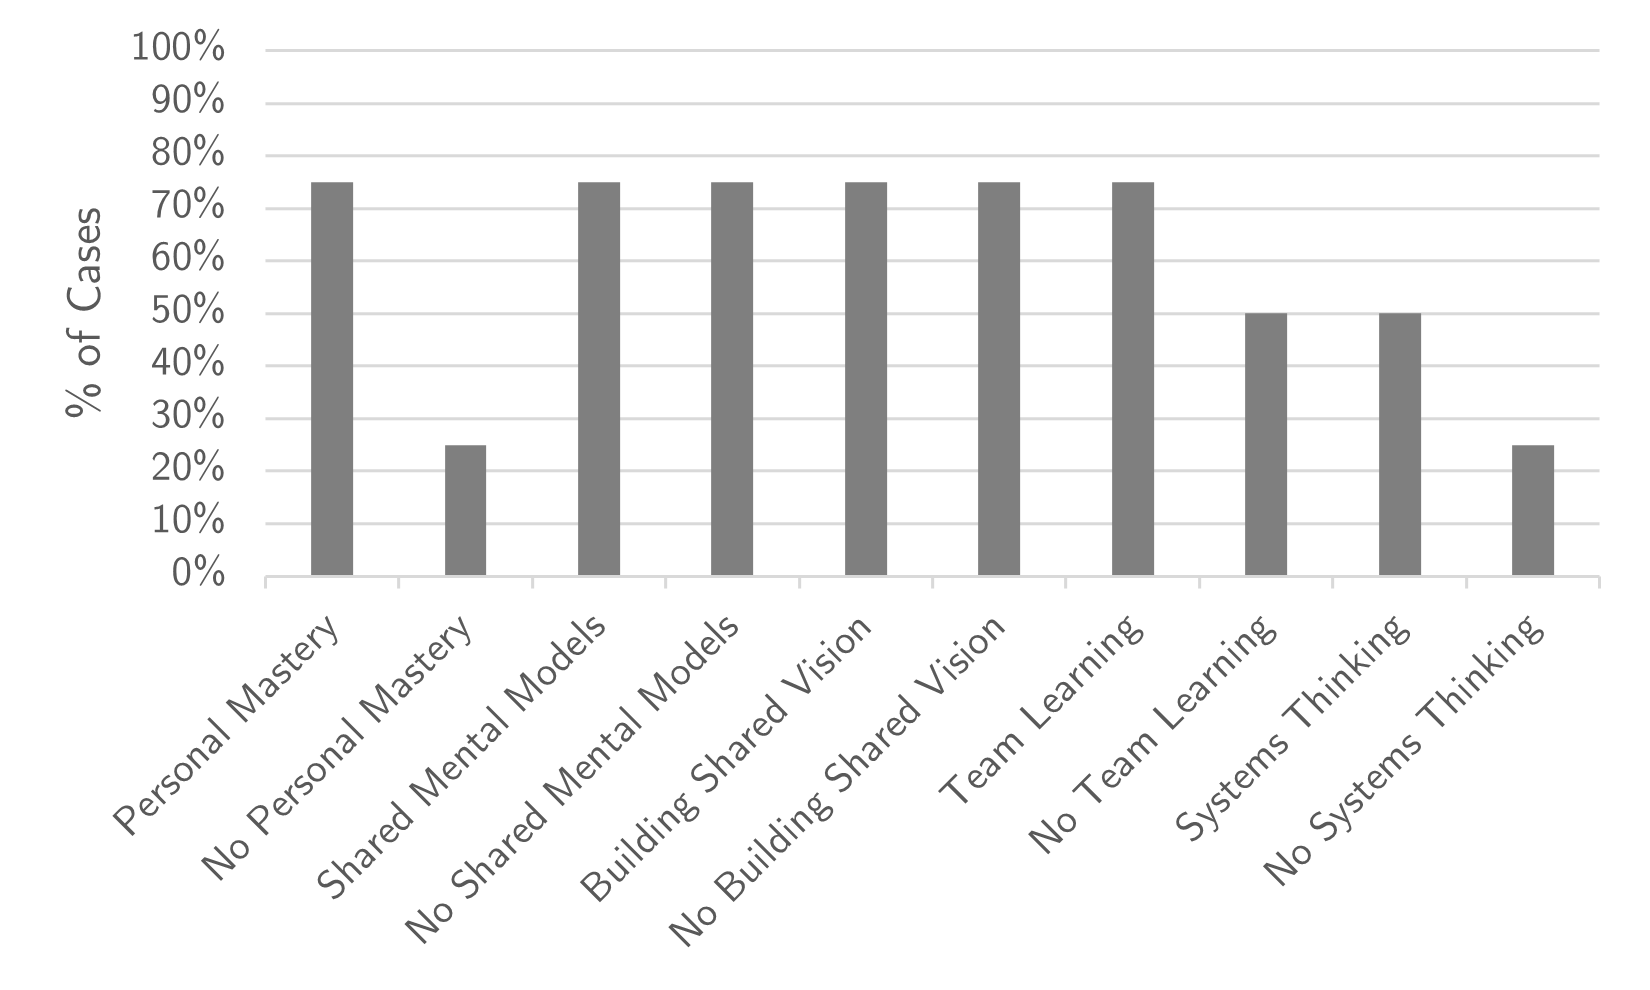
\includegraphics[width=0.95\linewidth]{images/learningorganisation_cases}
		\caption{Learning Organisation \% of Cases}
		\label{fig:learningorganisationcases}
	\end{subfigure}
	\caption{Interview results Learning Organisation}
	\label{fig:learningorganisationsantifragile}
\end{figure}


\subsection{Enterprise Architecture schools of thought}
\begin{figure}[H]
	\centering
	\begin{subfigure}[H]{0.5\textwidth}
		\centering
		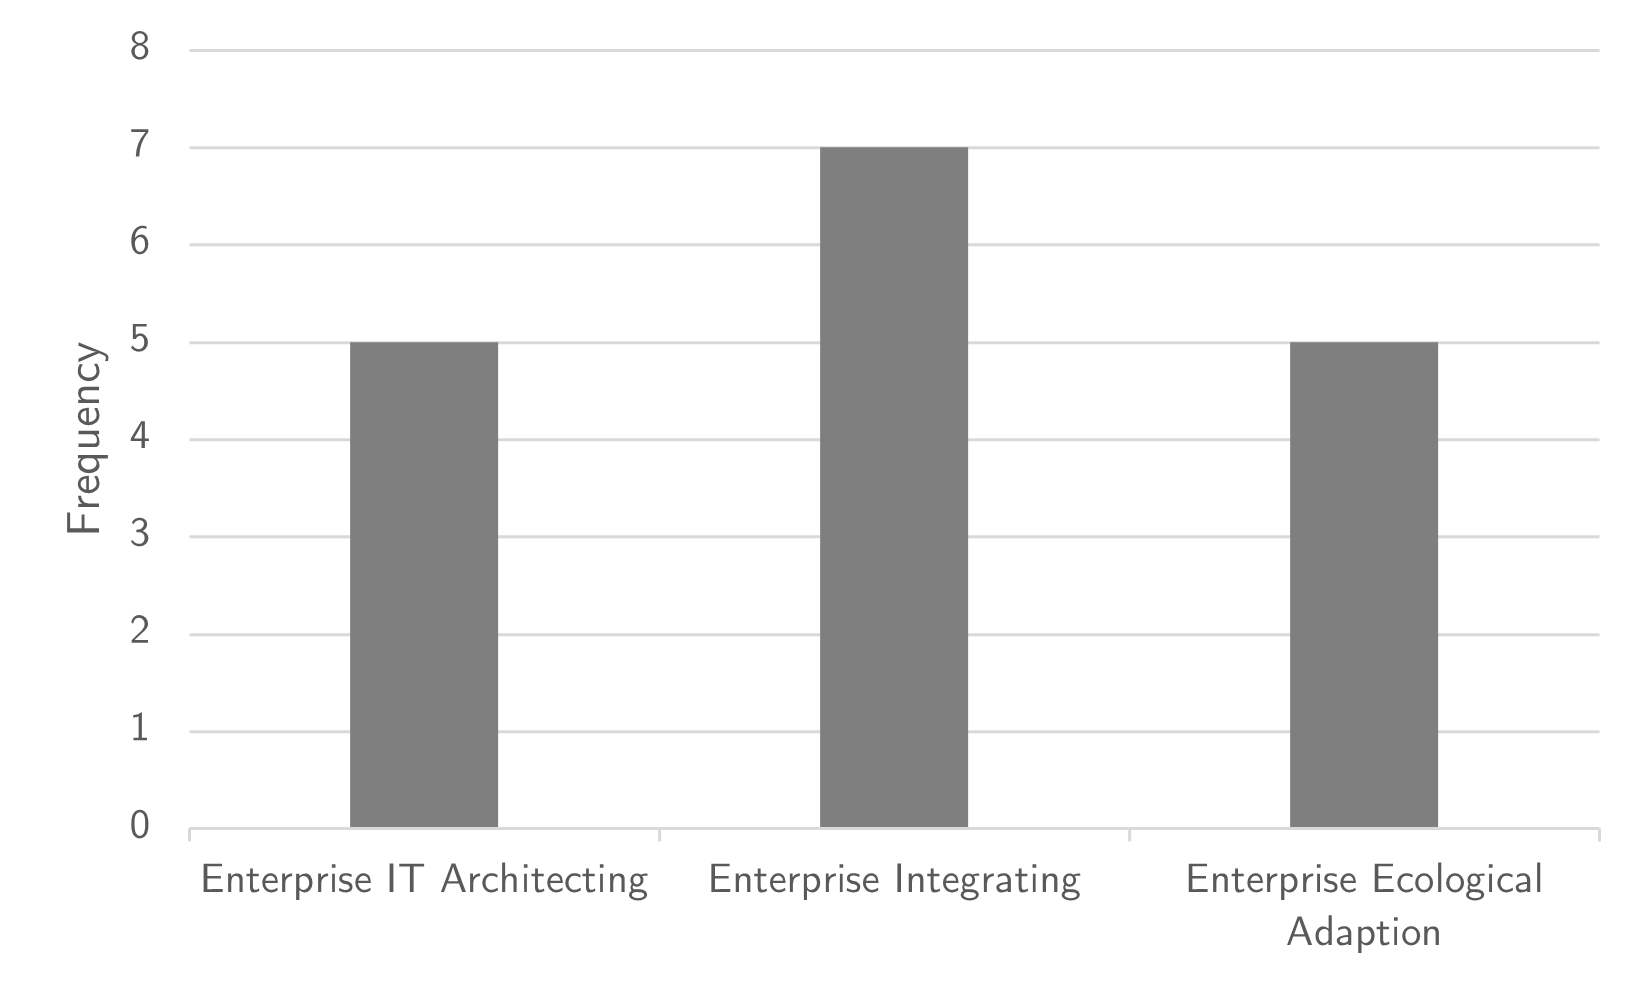
\includegraphics[width=0.95\linewidth]{images/easchools_frequency}
		\caption{Enterprise Architecture Schools of thought Frequency}
		\label{fig:easchoolsfrequency}
	\end{subfigure}%
	\begin{subfigure}[H]{0.5\textwidth}
		\centering
		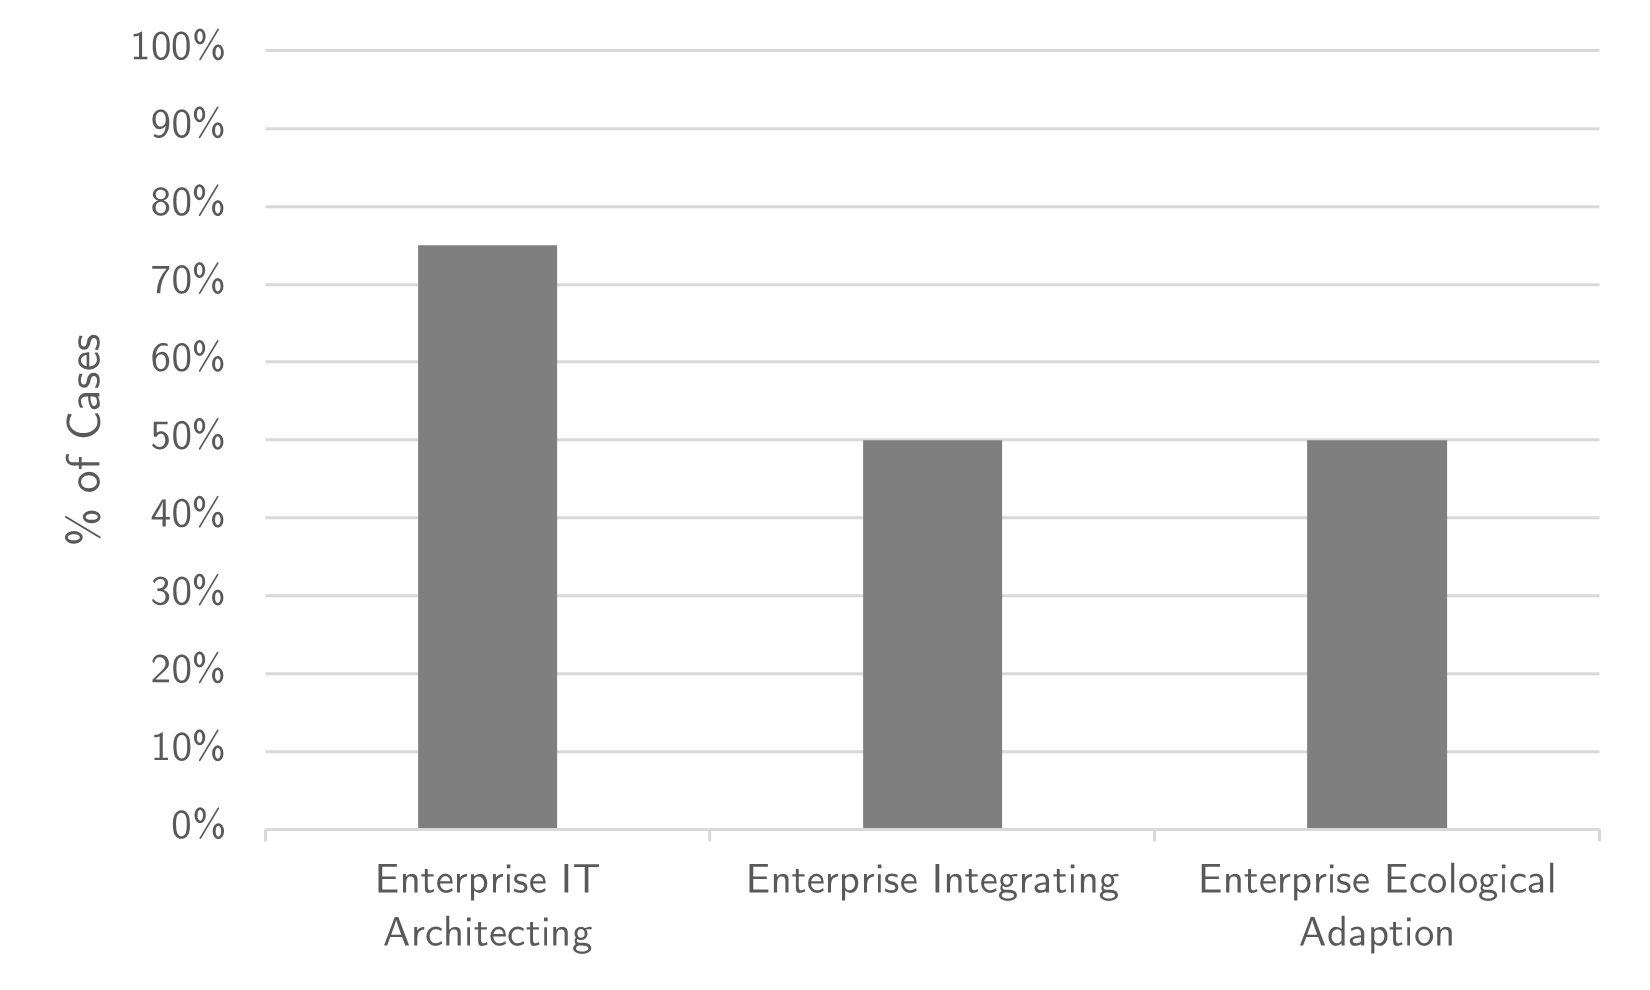
\includegraphics[width=0.95\linewidth]{images/easchools_cases}
		\caption{Enterprise Architecture Schools of thought \% of Cases}
		\label{fig:easchoolscases}
	\end{subfigure}
	\caption{Interview results Enterprise Architecture Schools of thought}
	\label{fig:easchoolsantifragile}
\end{figure}


\subsection{Findings}
\begin{figure}[H]
	\centering
	\begin{subfigure}[H]{0.5\textwidth}
		\centering
		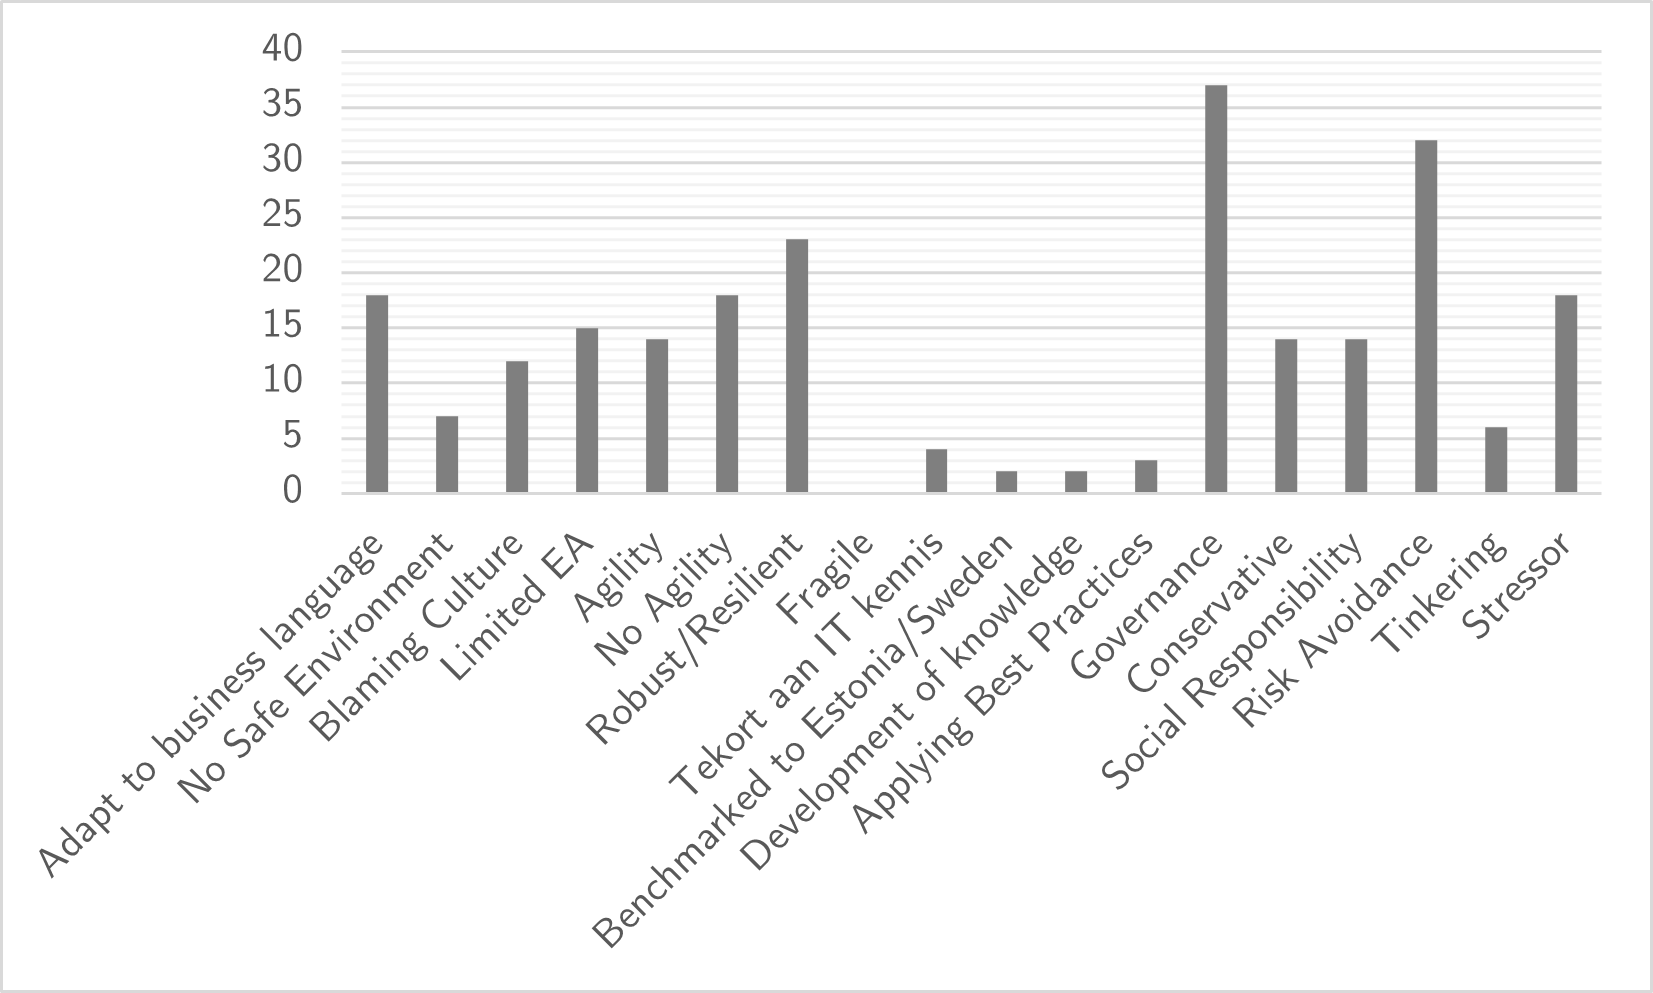
\includegraphics[width=0.95\linewidth]{images/findings_frequency}
		\caption{Findings Frequency}
		\label{fig:findingsfrequency}
	\end{subfigure}%
	\begin{subfigure}[H]{0.5\textwidth}
		\centering
		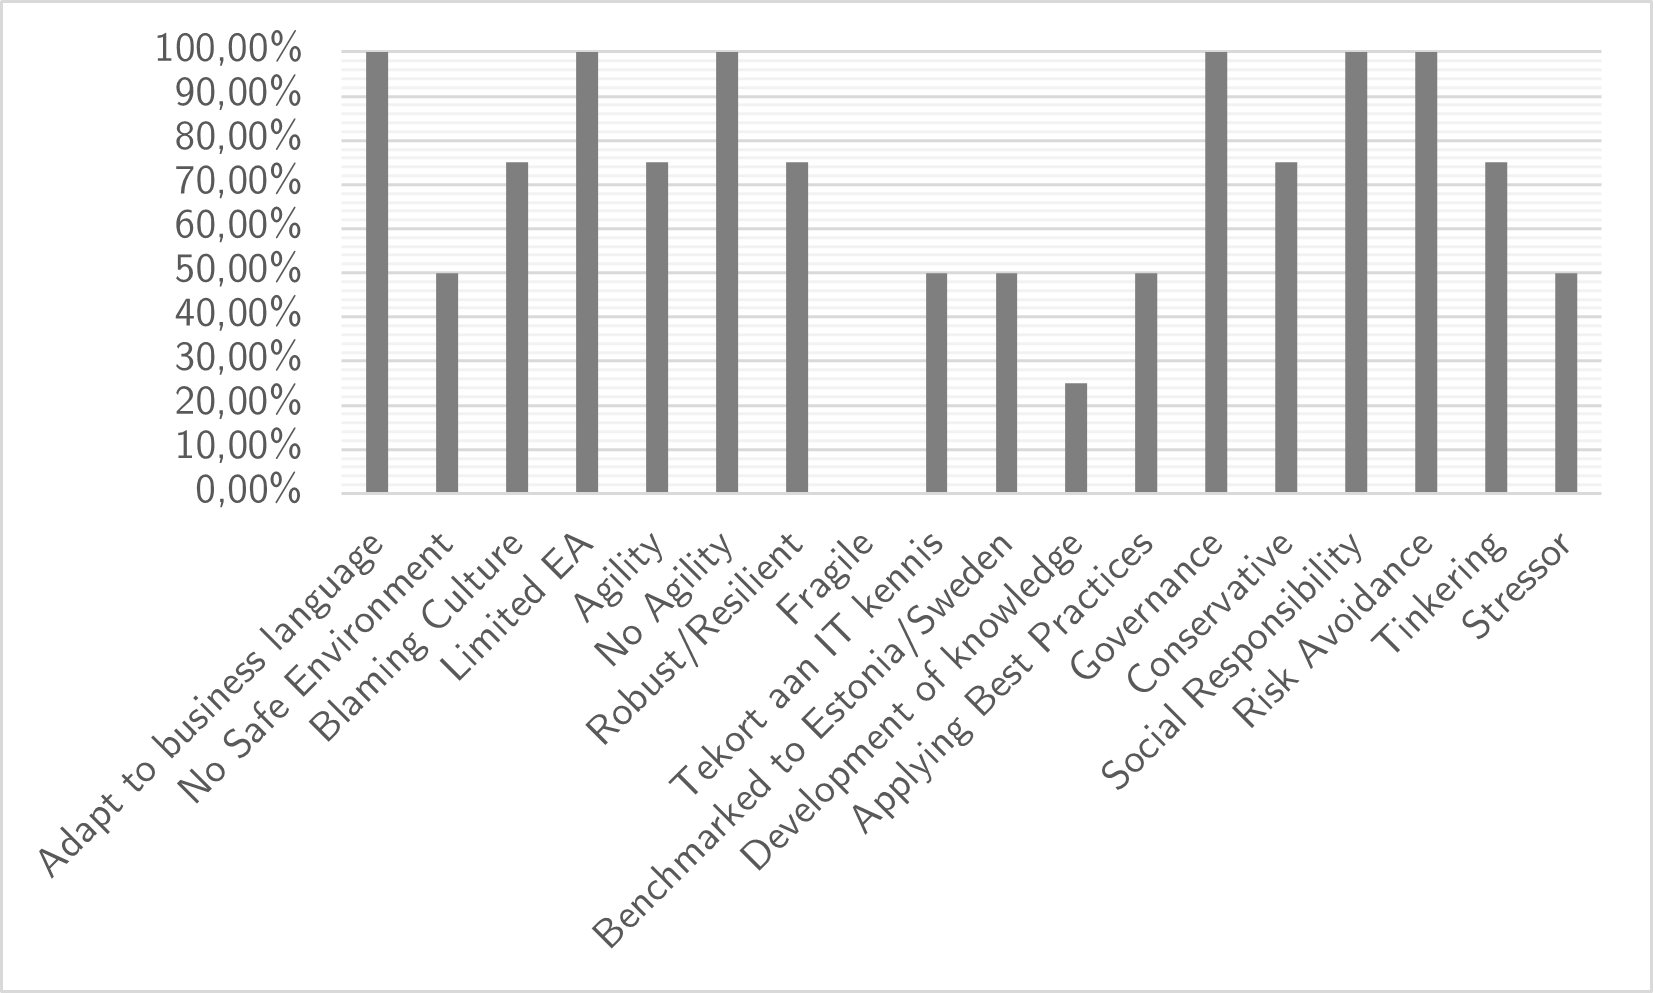
\includegraphics[width=0.95\linewidth]{images/findings_cases}
		\caption{Findings \% of Cases}
		\label{fig:findingscases}
	\end{subfigure}
	\caption{Interview results Findings}
	\label{fig:interviewresultsfindings}
\end{figure}


\section{Identified success factors}

\label{sec:interviewidentifiedsuccessfactors}
\begin{table}[!h]
	\begin{center}
		%\resizebox{\textwidth}{!}{%
			\begin{tabular}{@{}llllll@{}}
				%\toprule
				\textbf{Attribute} & \textbf{Behaviour} & \rot{90}{\textbf{Central Government}} & \rot{90}{\textbf{Local Government}} & \rot{90}{\textbf{Independent Software Vendor}} & \rot{90}{\textbf{Service Provider}} \\ \midrule
				Top Down C\&C & Engineering Resilience & \checkmark & \checkmark & \checkmark & \checkmark \\
				Micro-Management & Engineering Resilience & & & & \\
				Redundancy & Systems Resilience & & & & \\
				Modularity & Systems Resilience & & & & \\
				Loosely coupled & Systems Resilience & & & & \\
				Diversity & \acrshort{cas} Resilience & & & & \\
				Optionality & \acrshort{cas} Resilience & & & & \\
				Non-Monotonicity & \acrshort{cas} Resilience & & & & \\
				Emergence & \acrshort{cas} Resilience & & & & \\
				Self-Organisation & \acrshort{cas} Resilience & & & & \\
				Insert low-level stress & \acrshort{cas} Resilience & & & & \\
				Network-connections & \acrshort{cas} Resilience & & & & \\
				Fail Fast & \acrshort{cas} Resilience & & & & \\
				\Gls{resourcestoinvest} & Antifragile & & & & \\
				\Gls{senecabarbell} & Antifragile & & & & \\
				\Gls{insertrandomness} & Antifragile & & & & \\			
				\Gls{reducenaiveintervention} & Antifragile & & & & \\
				\Gls{skininthegame} & Antifragile & & & & \\
				\Gls{personalmastery} & Learning Organisation & & & & \\
				\Gls{sharedmentalmodels} & Learning Organisation & & & & \\
				\Gls{buildingsharedvision} & Learning Organisation & & & & \\
				\Gls{teamlearning} & Learning Organisation & & & & \\
				\Gls{systemsthinking} & Learning Organisation & & & & \\
				\bottomrule
			\end{tabular}
		%}
		\caption{Identified success factors from interviews}
	\end{center}
\end{table}

\section{Findings}

The central government is mostly robust and has a high risk aversion. With the administrative bodies of the local government the risk aversion is less and there is more insert low level stress. Because of this the local government is used to all the stressors and more antifragile.

\begin{remark}
Needs better description
\end{remark}